\section{Aplikace}
Aplikace je napsaná v nativní C++-14 ve vývojovém prostředí Visual Studio 2015. Jedná se o multiplatformní konzolovou aplikaci, která je primárně určena pro systémy ARM. 

Její obsluha je jednoduchá a funguje na bázi argumentů, které určují její chování. Nastavení parametrů se provádí přes externí soubor, což umožňuje jednodušší a pohodlnější manipulaci s aplikací. Disponuje širokým spektrem nástrojů od testování klasifikátorů, po jejich trénování až po samotnou detekci. Její nástroje jsou popsány v následujících podkapitolách.


 \begin{figure}[H]
\centering
\includegraphics[width=14cm]{figures/alg_moghog}
\caption{Algoritmus aplikace při selekci kombinace MoG a HoG detekce}
\label{mog_algorithm}
\end{figure}

Obrázek \ref{mog_algorithm} ilustruje průběh algoritmu při volbě detekce pomocí HoGu a MoGu. Prvním krokem algoritmu je získání snímku z aktuální videosekvence nebo kamery, pokud obrázek je prázdný cyklus zde končí. Snímek se následně předzpracovává převodem do stupně šedi a aplikací rozostřovacího filtru. Tento obrázek je následně zpracováván metodikou substrakcí pozadí a na tento obraz se aplikuje eroze a dilatace, to proto, aby se v snímku vyfiltrovaly malé nevýznamné oblasti a následně spojily ty větší potencionální oblasti. Tyto oblasti se obalí kontury a převedou se na rámečky. Díky těmto rámcům se z obrazu vystřihnou a získáme výstřižky, na kterých v následujícím kroku probíhá samotná detekce. Detekční metoda vrátí rámce potencionálních oblastí chodců a vykreslí se do původního obrazu a proces se opakuje do té doby, pokud získaný obrázek z kamery není prázdný. Pokud obrázek po aplikování masky substrakce pozadí neobsahuje dostatečně velké oblasti k aplikaci rámců, program pokračuje načítáním dalšího rámce z kamery.  

\subsection{Testování klasifikátoru}
Testování klasifikátoru dle jejich parametrů vůči nějaké sadě negativních a pozitivních dat je nedílnou součástí vytvoření ideálního a úspěšného klasifikátoru.  Aplikace nabízí testování OpenCV a Dlib klasifikátoru. Diskriminační klasifikátor SVM z OpenCV lze testovat třemi způsoby. První a náhodný přístup je generování parametrů a různou iterací.

Další efektivnějším způsobem je testování pomocí diferenciální evoluce. Tento algoritmus vychází z genetického žíhání. Algoritmus nastaví určitý počet dimenzí pro testování parametrů SVM a následně probíhá ``žíhání'' parametrů takřka k jejich dokonalosti. Tento proces trvá 1000 cyklů.

Posledním druhem testování pro klasifikátor SVm z OpenCV je obdobné z Dlib knihovny, jedná se o vnořené cykly, kde se hrubou silou postupně testují parametry. 

Pro klasifikátor z Dlib knihovny je použita pouze metodika pro postupné testování parametrů hrubou silou v cyklech. Výhodou této metodiky je rozdělení trénovacích dat do 3 množin, kde dvě slouží na trénování a jedna pro testování a následně naopak. Toto testování trvá velice dlouho a výsledkem jsou přesnosti pro pozitivní a negativní množinu dat.


\subsection{Trénování klasifikátoru}
Program také umožňuje natrénování vlastního klasifikátoru. Parametry se vyberou z externího souboru s nastavením. V tomto souboru jsou také uloženy cesty k souborům se vzorky. 

Trénovací režim aplikace lze spustit přes argument '-t=train" a následně je uživateli nabídnut typ trénování. Program zvládne vytrénovat klasifikátor jak z knihovny OpenCV, tak i z knihovny Dlib. 

Trénování klasifikátorů z OpenCV probíhá naplněním vzorků do paměti včetně jejich kategorizace. Následně pro každý vzorek jsou vypočítané jeho vlastnosti a opět uložený do paměti programu. Posledním krokem před trénováním je jejich převod do jednořádkové matice a poté je spuštěno samotné trénování klasifikátorů. Tento krok trvá v závislosti na velikosti trénovací matice a zvolených parametrů. Uživatel může zvolit i dvojité trénování, za tímto stojí stejný postup, ale na konci trénování se spustí detekce pomocí posuvného okénka na negativních vzorcích a tyto vzorky budou rozšířeny o výstup z detektoru. Tento proces se nazývá Bootstraping. Výstupem trénování je soubor YAML, který je čitelný a slouží pro serializaci strukturovaných dat. Nalezneme zde parametry, použité pro trénování, vytrénované vzorky a vektor, který určuje rozdělující přímku.

Další možností je vytrénovaní klasifikátoru z knihovny Dlib. Trénování je obdobné jako u předchozí metody. Data jsou načtena jako mapy obrázků a tyto obrázky se parsují pomocí XML souboru. Trénování probíhá pouze z pozitivních vzorků a vychází z \cite{hog:dalal}. Výstupem je soubor s příponou dat.

Poslední možností trénování je kombinace výše zmíněných postupů. Vzorky se zpracují za pomocí OpenCV knihovny a vstupem do trénovací metody klasifikátoru z Dlibu je trénovací matice. Tu je nejprve nutné převést na formát této knihovny a poté je možné provést trénování.

Podstatný rozdíl mezi těmito binárními klasifikátory je v rozdílu jejich štítků. OpenCV klasifikátor můžeme definovat štítky libovolně, nejčastější však 1 pro pozitivní vzorky a 0 pro negativní. Zatím co Dlib klasifikátor přijímá pouze 1 pro pozitivní a zápornou 1 pro negativní vzorky.

Trénování klasifikátoru je velmi náročnou  operací na hardwarové prostředky. Ovšem závisí na trénovací sadě. Sada o počtu 200 tisíc vzorků zkonzumuje až 16 GB paměti.  Trénování kaskádového klasifikátoru je povoleno jen na  64-bitovém Windows, protože k trénování je využívána externí OpenCV aplikace. 

\subsection{Anotace chodců v obraze}
Aplikace také disponuje nástrojem pro anotaci chodců v obraze. Najednou umožňuje anotovat až 5 chodců a tyto anotace, i když to není až tak potřebné pro správnost anotace, jsou od sebe barevně odlišeny. Manipulace s tímto nástrojem je velmi snadná a jeho náhled je na obrázku \ref{tool_anotate}.

Klávesami `0' až `4' se přepíná mezi anotacemi, přičemž se tato selekce vypíše pro kontrolu do konzole. Klávesa `r' slouží pro vynulování vybrané anotace. Klávesou `n' přeskočíme aktuální snímek bez uložení anotovaných pozic. Klávesa `s' uloží aktuální anotované pozice do paměti a přepne se na další snímek, přičemž pozice první anotace zůstane nezměněná, to umožňuje jednodušší práci, pokud se v obraze nachází jen jeden chodec. Klávesy `i', `j', `k' a `l' umožňuje pohyb v obraze, pro přesnější umístění anotované části. Pokud tyto klávesy stiskneme společně s klávesou `shift', umožní nám to měnit velikost dané anotace. Klávesa `x' uloží aktuální pozice anotací v paměti do souboru. Tato funkcionalita umožňuje přerušovanou práci na anotacích videosekvence, ale vyžaduje manuální úpravu souboru uživatelem. Anotovaná část se může překrývat s jinou. Konkrétní anotace je zobrazena pro kontrolu samostatně zobrazena v dalším okně.

Všechny tyto oblasti zájmu a snímek s anotacemi jsou uloženy na disk v podobě obrázku pro pozdější kontrolu nebo oblasti zájmu mohou být použity pro trénování nebo cross validaci klasifikátoru. Výstup tohoto nástroje je plně kompatibilní s evaluační funkcí programu a jedná se tady o GroundTruth soubor všech anotací ve videosnímku.
 \begin{figure}[H]
\centering
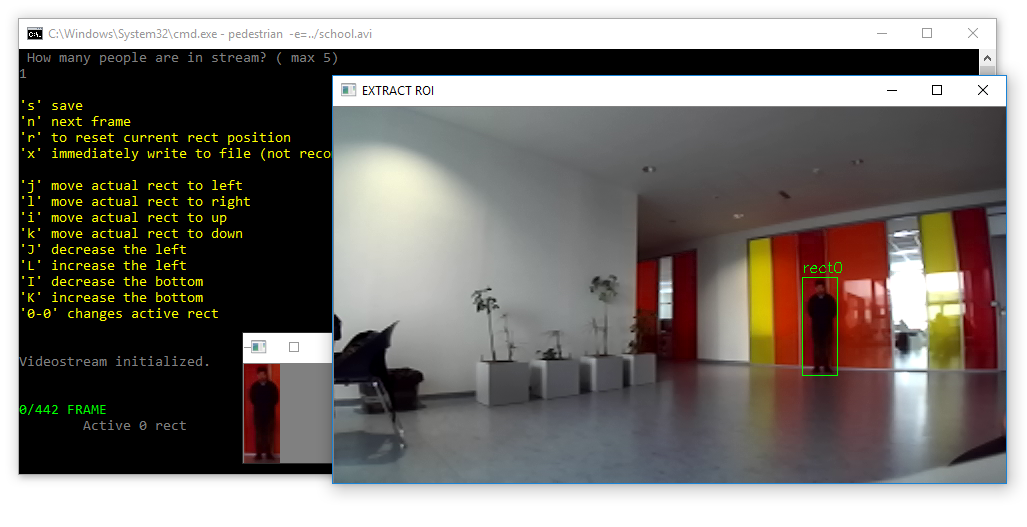
\includegraphics[width=15cm]{figures/annotation_example}
\caption{Nástroj pro anotování oblastí chodců}
\label{tool_anotate}
\end{figure}

\subsection{Tvorba negativních vzorků z obrazu}
Tento nástroj umožňuje vytvořit negativní vzorky pro trénování procházením obrázku pomocí posuvného okénka. Velikost posuvného okénka je definována v externím souboru. Vstupem je textový soubor s cestami k obrázkům.
